% This file was created with tikzplotlib v0.10.1.
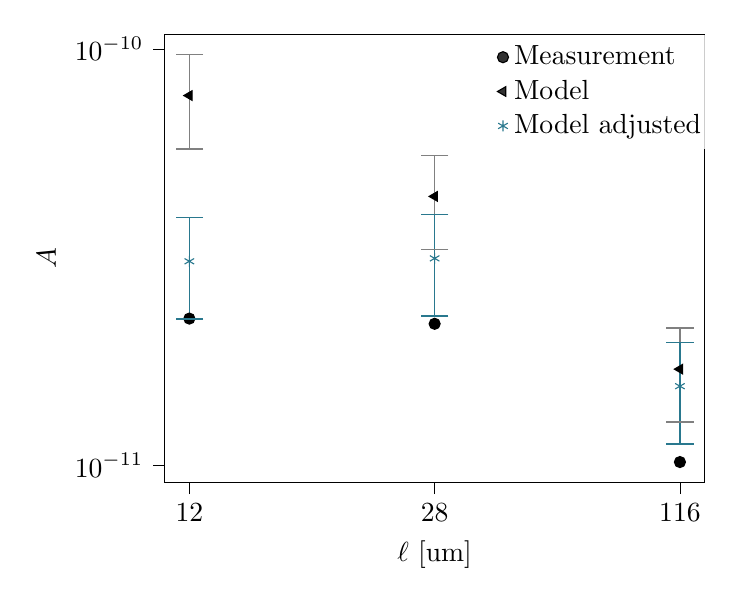
\begin{tikzpicture}

\definecolor{darkgray176}{RGB}{176,176,176}
\definecolor{gray}{RGB}{128,128,128}
\definecolor{teal41120142}{RGB}{41,120,142}

\begin{axis}[
legend cell align={left},
legend style={
  fill opacity=0.8,
  draw opacity=1,
  text opacity=1,
  at={(0.6,1)},
  anchor=north west,
  draw=none
},
log basis y={10},
tick align=outside,
tick pos=left,
x grid style={darkgray176},
xlabel={\(\displaystyle \ell\) [um]},
xmin=-0.1, xmax=2.1,
xtick style={color=black},
xtick={0,1,2},
xtick={0,1,2},
xtick={0,1,2},
xtick={0,1,2},
xtick={0,1,2},
xticklabels={12,28,116},
xticklabels={12,28,116},
xticklabels={12,28,116},
xticklabels={12,28,116},
xticklabels={12,28,116},
y grid style={darkgray176},
ylabel={\(\displaystyle A\)},
ymin=9.10458557707837e-12, ymax=1.08528817324762e-10,
ymode=log,
ytick style={color=black},
ytick={1e-13,1e-12,1e-11,1e-10,1e-09,1e-08},
yticklabels={
  \(\displaystyle {10^{-13}}\),
  \(\displaystyle {10^{-12}}\),
  \(\displaystyle {10^{-11}}\),
  \(\displaystyle {10^{-10}}\),
  \(\displaystyle {10^{-9}}\),
  \(\displaystyle {10^{-8}}\)
}
]
\addplot [draw=black, fill=black, mark=*, only marks]
table{%
x  y
0 2.25195947100078e-11
1 2.1881000070955e-11
2 1.01901886166217e-11
};
\addlegendentry{Measurement}
\addplot [draw=black, fill=black, mark options={rotate=90}, mark=triangle*, only marks]
table{%
x  y
0 7.72866725493358e-11
1 4.42492174441183e-11
2 1.70315215247974e-11
};
\addlegendentry{Model}
\addplot [draw=teal41120142, fill=teal41120142, mark=asterisk, only marks]
table{%
x  y
0 3.09146690197343e-11
1 3.1416944385324e-11
2 1.54986845875656e-11
};
\addlegendentry{Model adjusted}
\path [draw=gray, semithick]
(axis cs:0,5.76065526194191e-11)
--(axis cs:0,9.69667924792524e-11);

\path [draw=gray, semithick]
(axis cs:1,3.29816873851768e-11)
--(axis cs:1,5.55167475030598e-11);

\path [draw=gray, semithick]
(axis cs:2,1.26946497829973e-11)
--(axis cs:2,2.13683932665974e-11);

\addplot [semithick, gray, mark=-, mark size=5, mark options={solid}, only marks, forget plot]
table {%
0 5.76065526194191e-11
1 3.29816873851768e-11
2 1.26946497829973e-11
};
\addplot [semithick, gray, mark=-, mark size=5, mark options={solid}, only marks, forget plot]
table {%
0 9.69667924792524e-11
1 5.55167475030598e-11
2 2.13683932665974e-11
};
\path [draw=teal41120142, semithick]
(axis cs:0,2.24573463417858e-11)
--(axis cs:0,3.93719916976828e-11);

\path [draw=teal41120142, semithick]
(axis cs:1,2.28222142896456e-11)
--(axis cs:1,4.00116744810024e-11);

\path [draw=teal41120142, semithick]
(axis cs:2,1.12587111122838e-11)
--(axis cs:2,1.97386580628474e-11);

\addplot [semithick, teal41120142, mark=-, mark size=5, mark options={solid}, only marks, forget plot]
table {%
0 2.24573463417858e-11
1 2.28222142896456e-11
2 1.12587111122838e-11
};
\addplot [semithick, teal41120142, mark=-, mark size=5, mark options={solid}, only marks, forget plot]
table {%
0 3.93719916976828e-11
1 4.00116744810024e-11
2 1.97386580628474e-11
};
\end{axis}

\end{tikzpicture}
